%!TEX root = main.tex

\section{System measurement}
\label{sec:system-measurement}

We will use the TCP traces collected on the front-end server to measure our crowdsourced live video system in the wild. The connections between front-end server and storage system go through large bandwidth and small RTT internal network so they are stable in our system.  In this section we do not analysis TCP connections in internal network but just the connections that go through WAN. In Secion~\ref{sub:upload-analysis} we will analysis the TCP connection between camera and front-end server which is used to upload video to front-end server. In Secion~\ref{sub:download-analysis} we will analyse the TCP connection between viewers and front-end server which is used to download video from front-end sever. And in Secion~\ref{sub:relationship-analysis} we will analyze the relationship between the upload and download connections and try to figure out how the upload process influences the whole system performance.

\subsection{Upload TCP connection analysis}
\label{sub:upload-analysis}
Cameras upload video to front-end server once they produce frame. The fluency of upload video directly influences the watching experience of viewer. Two factors may influence the upload process: one is the interval of frame produced process and the other is the delay by the network. We define \emph{TCP stall} as an event where the duration between two consecutive packets received/sent by the sender is larger than $\min(\tau\cdot\text{SRTT}, \text{RTO})$. We set $\tau$ to 2 in this work as the TCP sender could at least receive or send one packet during $2RTT$ in the ideal condition. And as in the upload flow we can get the RTT of this flow just in the 3WHS (3-way handshake) process, we use the RTT in 3WHS as the \text{SRTT} for this flow. 

As we just capture packets of TCP flows at the front-end server, for upload flow it is not possible to distinguish the reorder packet and the real loss packet. At the point of front-end server ,all of them look like reordering packets. We define the stalls that happen when receiving reordering packet as reorder stall and other stalls as normal stall. When the camera does not send any data to the front-end server and also does not send FIN to finish this connection the front-end sever will send keep-alive packets to keep this connection alive. In our system we set the keep-alive packet's sending out interval as 5 seconds. And we define this stall as keep alive stall. We find that all the stall time accounts for 31.6\% of all the upload flow time, and among these stalls 93.5\% stall is normal stall, 1.3\% is reorder stall while 5.2\% is keep alive stall. That means the packet loss or reorder caused by the network is not the main factor that influence the rate of upload flow. However, the interval of frame produced process is the main factor that influence the upload flow. That can also be confirmed by the fact that the upload flow's rate is just 60KB/s, much smaller than the upload bandwidth. 

\iffalse
 The percentage of different stall time is shown in Table~\ref{tbl:upload-stall}.

\begin{table}[ht]
\tablefontsize
\renewcommand{\arraystretch}{\assize}
 \setlength{\tabcolsep}{3pt}
\caption{Percentage of different stall in upload flows.}
\centering
\begin{tabular}{c|c}
	\toprule
	 type & percentage(\%) \\
	\hline
	normal & 93.5 \\
	\hline
	reorder & 1.3 \\
	\hline
	keep alive & 5.2 \\
	\bottomrule
\end{tabular}
\label{tbl:upload-stall}
\termspace
\end{table} 

From Table~\ref{tbl:upload-stall}, we can see that 93.5\% stall is normal stall while the reorder stall is just 1.3\%. 
\fi

We further find that the total frame's reorder rate is 1\% and among the reorder packets 6\% suffer from timeout reorder. If the packet in upload flow is lost and can not be recovered by fast retransmit, the front-end server will receive a timeout reorder packet. We define the reorder packet as timeout reorder packet if the interval between the reorder packet and the last send-in data is larger than 0.2 second(the minimum RTO in linux kernel). 

\iffalse
\begin{table}[ht]
\tablefontsize
\renewcommand{\arraystretch}{\assize}
\setlength{\tabcolsep}{3pt}
\caption{Reorder packets rate in upload flows.}
\centering
\begin{tabular}{c|c}
	\toprule
	reorder rate & timeout/reorder \\
	\hline
	1\% & 6\% \\
	\bottomrule
\end{tabular}
\label{tbl:reorder-rate}
\termspace
\end{table} 
\fi

Although the packet loss or reorder is not the main factor that influences the upload flow rate, we find that packet reorder rate greatly influence the upload flow size, especially when the reorder rate becomes large. Table~\ref{tbl:reorder-rate-influence} shows the influence of reorder rate to upload flows. As reorder rate grows, the upload flows' flow rate, flow size and FCT(Flow Complete Time) become small. Especially when the reorder rate is larger than 20\% which means the network environment is very bad, the upload flow size becomes as small as 0.73MB, much smaller than the flow size(5.1MB) when the reorder rate is 0-10\%. The video provider also views the video that he uploads. If the upload network environment is bad and the reorder packets rate becomes high, the provider may terminal the upload process because the viewing experience is bad. That is why the flow size suddenly drops when the reorder rate becomes large. 

\begin{table}[ht]
\tablefontsize
\renewcommand{\arraystretch}{\assize}
 \setlength{\tabcolsep}{3pt}
\caption{Influence of different reorder packets rate to upload flows.}
\centering
\begin{tabular}{c|c|c|c}
	\toprule
	 reorder rate & flow rate & flow size & FCT\\
	\hline
	0-10\% & 64KB/s & 5.1MB & 87.7s \\
	\hline
	10-20\% & 48KB/s & 4.7MB & 72.8s \\
	\hline
	$>$20\% & 17KB/s & 0.73MB & 60.7s \\
	\bottomrule
\end{tabular}
\label{tbl:reorder-rate-influence}
\termspace
\end{table}  

\subsection{Download TCP connection analysis}
\label{sub:download-analysis}

\subsubsection{Stall analysis}
\label{sub:stall-download}

To figure out what factors influence the download flows between front-end server and viewers, we analyze the stalls in the download TCP flow. We define the stall as the same in Section~\ref{sub:upload-analysis}. As the front-end server can get the ACK from viewers, we can calculate RTT dynamically in download flow. 
According the positions that the stall happens we can define the stall as the following type. \emph{timeout retrans} is the stall that is caused by the timeout retransmission. \emph{resource constraint} happens when there are not data to send and that is often caused by that the camera does not upload data timely(the same with the normal stall in Section~\ref{sub:upload-analysis}). \emph{packet delay} is caused when the ACK packets are delayed to come back, either by network or client. When the viewers do not have enough buffer to handle the data and reduce its rwnd to zero the front-end server can not send any data until the viewers extend its rwnd. Such stall is defined as \emph{zero rwnd} stall. When there are not data to send for a long time and the viewers do not stop this connection, every 5 seconds the front-end server will send keep-alive packets to keep this connection alive. We define such stall as \emph{keep alive} stall. In totally we find that all the time of stall account for 35.2\% of all the download flow time.  Table~\ref{tbl:stall-download} shows the percentage of different stalls in download flow.

\begin{table}[ht]
\tablefontsize
\renewcommand{\arraystretch}{\assize}
 \setlength{\tabcolsep}{3pt}
\caption{Percentage of different stalls in download flow.}
\centering
\begin{tabular}{c|c}
	\toprule
	 type & percentage(\%)\\
	\hline
	resource constraint & 39.4   \\
	\hline
	packet delay & 8.2 \\
	\hline
	zero rwnd & 16.3 \\
	\hline
	keep alive & 10.1 \\
	\hline
	timeout retrans. & 22.8 \\
	\hline
	unknown & 1.5 \\
	\bottomrule
\end{tabular}
\label{tbl:stall-download}
\termspace
\end{table}  

From Table~\ref{tbl:stall-download} we can see that the \emph{resource constraint} accounts for 39.4\% of all the download stall which is the largest part. That is partly caused by the upload flows. In Section~\ref{sub:upload-analysis}we find that stalls account for 31.6\% of all upload flow time. As the camera stop sending data(caused by frame produce terminal) for a while, the front-end server does not have data to send. 16.3\% stall is \emph{zero rwnd} stall, which means the viewers' process ability is also an important factor to influence the efficiency of the system. \emph{keep alive} stall accounts for 10.1\% of download stall time which means that there are consumers who still wait for some time to stop the connection even when the producer stop posting video. 22.8\% stall is \emph{timeout retrans} which is caused by the network. In Section~\ref{sec:frame-analysis} we will further analysis the timeout retransmission in detail.

\subsubsection{Variety of RTT}
\label{sub:RTT}

RTT is an important factor that influences the flow rate. The flows with small RTT are more likely to get high flow rate. RTT is determined by two factors. One is the number of hops between two nodes which is controlled by the route algorithm. The other is the packets' cache time at the routers which is controlled both by the router buffer capacity and the volume of packets in the network. In the WAN(Wide Area Network), the route algorithm and router buffer capacity are out of the control of sever. The only way that the server can control the RTT is by controlling the packets that is sent to the network.

In table~\ref{tbl:inflight-rtt} we analysis the change of RTT when the $in\_flight$ change. $in\_flight$ is the number of packet in-flight which is defined as the following equation:

\begin{footnotesize}
 \begin{equation}
\label{eq:conserve}
\begin{aligned}
in\_flight = \enspace & packets\_out + retrans\_out \enspace - \\
& (sacked\_out + lost\_out) \enspace ,
\end{aligned}
\end{equation}
\end{footnotesize}

where $packets\_out$ is the number of packets between $snd\_una$ (the packet with highest sequence number the receiver has acknowledged) and $snd\_nxt$ (the next new segment the sender would transmit), $retrans\_out$ is the number of retransmitted but not yet acknowledged packets, $sacked\_out$ is the number of SACKed packets, and $lost\_out$ is the number of lost packets.

We examine the change of RTT by comparing it with the RTT which is calculated in the 3-way handshake(3WHS) phase(referred to as 3WHS\_RTT). From table~\ref{tbl:inflight-rtt} we can see that as the $in\_flight$ becomes large, the RTT also becomes large. When the $in\_flight$ becomes as large as 64KB, the RTT is even 2.6 times of the 3WHS\_RTT. That means when the $in\_flight$ become large the routers need more time to deal with the coming packets and that results in large RTT.      

\begin{table}[ht]
\tablefontsize
\renewcommand{\arraystretch}{\assize}
 \setlength{\tabcolsep}{3pt}
\caption{The varity of RTT when the $in\_flight$ packets changes.}
\centering
\begin{tabular}{c|c}
	\toprule
	 $in\_flight$ & RTT/3WHS\_RTT \\
	\hline
	$<$4KB & 0.89 \\
	\hline
	4KB-8KB & 1.08  \\
	\hline
	8KB-16KB & 1.31  \\
	\hline
	16KB-32KB & 1.38  \\
	\hline
	32KB-64KB & 1.61 \\
	\hline
	$>$64KB & 2.6  \\
	\bottomrule
\end{tabular}
\label{tbl:inflight-rtt}
\termspace
\end{table}  


%\subsection{Storage TCP connection analysis}
%\label{sub:storage-analysis}
%In our live video system, when cameras upload video to front-end server it re-send it to the cassandra storage server to store the video. When the watch app request to view a video, the front-end server will fetch video from the cassandra storage server. For storage and fetching video on the cassandra, front-end server needs to setup two different TCP connections. At storage process, after front-end server send data to cassandra, cassandra will reply a message to the server to inform whether the data has been inserted successfully. At fetching process, front-end server send a key to cassandra, and then cassandra will reply data to front-end sever according the key. That means for both of storage and fetching connections, there are send-in and send-out data. In this section we will detail the  send-in and send-out data in both of two connections in detail. 

%\subsubsection{Storage process}
%\label{sub:storm}
%The send-out data in storage process is the data that need to store in cassandra, and the send-in data is the message to inform whether the data has been inserted successfully. Table~\ref{tbl:storage-data} shows the statistics in the storage process. From the table we can see that send-out data rate is small, just 35KB/s much smaller than the rate that the camera send data to front-end server. In our personal live video system, once the front-send server receives a image or voice frame from camera, it will storm the frame to cassandra. However when the front-end server sends out the frame to cassandra, it can not send next frame until it receives successful reply message from cassandra. 

%In DCN(Data Center Network) the packet loss rate is quite small, so the loss rate of send-out data is quite small, just 0.001\%. But surprisingly, we find that 69.8\% of the loss packets are recovered by timeout retransmission. After we analysis those timeout retransmission we find that all of them is caused by less pkt retransmission. As the front-end server can not send next frame until it receive the reply message, the packet in network often less than 3 packets(if the size of the frame is less than 3 packets). At such condition, the server can not receive enough dupacks to trigger fast retransmission.  

%As the send-in data just send reply message which is small and the time use to calculate the rate is the whole flow complete time, the rate of send-in is even samller than the send-out data, just 10KB/s. As the small packet loss rate and the one frame one reply charater of storage process, we can not find any reorder packets in send-in data.  
       
%\begin{table}[ht]
%\tablefontsize
%\renewcommand{\arraystretch}{\assize}
 %\setlength{\tabcolsep}{3pt}
%\caption{Send out and in analysis in storage process.}
%\centering
%\begin{tabular}{c|c|c|c}
%	\toprule
%	 type & rate & loss/reorder rate & timeout num/loss num \\
%	\hline
%	send-out & 35KB/s & 0.001\% & 69.8\% \\
%	\hline
%	send-in & 10KB/s & - & - \\
%	\bottomrule
%\end{tabular}
%\label{tbl:storage-data}
%\termspace
%\end{table} 

%\subsubsection{Fetching process}
%\label{sub:fetch}
%Once the watch-app send request to watch a live video, the front-end server begins to fetch data from cassandra. The cassandra store each image and voice frame individually, and each frame has an unique key. The front-end server fetch the frames of video one by one using their keys, and it will not fetch next frame util it successfully get a full frame. The send-out data in fetching data process is that the front-end server sends 'get data' message to cassandra, and the send-in data is that cassandra reply video frame to front-end server. Table~\ref{tbl:fetch-data} shows the statistics in the fetching process. From the table we can see that the rate in send-in data is 1.98MB/s, much larger than the rate of send-out in storming process. That is because the wathcing process is a little delay than the uploading data process of camera, which means the data has been stored in the cassandra. The reorder rate of the send-in data is also small, just 0.0124\%. And 33.2\% of the reorder packet is timeout retransmission data. We find that most of the timeout reorder packet is also less pkt retransmissio, similar with send-out data in storage process.

%Send-out data's rate is just 67KB/s, because the send-out data is small which just carries the request key. The loss rate is also small just 0.0125\%, but nearly all of the loss packets are recovered by timeout retransmission. That is because the send-out packets are the request packet carrying the key of the frame. Front-end server will not send out any data utill it receives the full frame. The loss packet can only recover by the timeout retransmission as there is only one packet in flight.  

%\begin{table}[ht]
%\tablefontsize
%\renewcommand{\arraystretch}{\assize}
% \setlength{\tabcolsep}{3pt}
%\caption{Send out and in analysis in fetch data process.}
%\centering
%\begin{tabular}{c|c|c|c}
%	\toprule
%	 type & rate & loss/reorder rate & timeout num/loss num \\
%	\hline
%	send-out & 67KB/s & 0.0125\% & 99.6\% \\
%	\hline
%	send-in & 1.98MB/s & 0.0124\% & 33.2\% \\
%	\bottomrule
%\end{tabular}
%\label{tbl:fetch-data}
%\termspace
%\end{table} 


\subsection{Relationship between TCP connections}
\label{sub:relationship-analysis}
In the above section, we discuss the connections in our system individually. These TCP connections also have influence to each other. For example the reorder in upload flows may cause the download flows do not have data to send. In this section we will detail the relationship between these TCP connections.

The system uses a unique ID for each video, so we can match the upload and download flow by the video ID. There are hundreds of front-end servers in our system, so the video may upload to a server while viewers may download it from other servers. Our data is collected from one server so we can not find upload flow for each download flow. Figure~\ref{fig:up-down-rate} shows the corresponding rate of upload and download flows who have the same ID. From the figure we find that the most of the spots are spread near the diagonal line which means that most videos' download flow rate is the same with the upload flow rate. This confirms that for the crowdsourced live video, the video produce and upload process are the key for viewers' experience.  

\begin{figure}[t]
\centering
\subfloat[The corresponding rate of upload and download flows.]{
	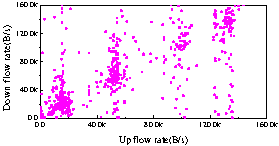
\includegraphics[width=1.8in]{up-down-rate}
	\label{fig:up-down-rate}}
\hspace{1em}%
\subfloat[The corresponding FCT of upload and download flows.]{
	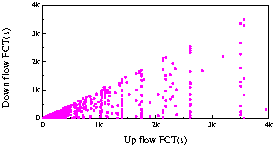
\includegraphics[width=1.8in]{up-down-fct}
	\label{fig:up-down-fct}}
	\hspace{1em}%
\subfloat[The corresponding download flow FCT with upload flow rate.]{
	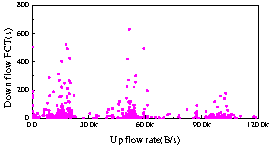
\includegraphics[width=1.8in]{up-rate-down-fct}
	\label{fig:up-rate-down-fct}}
\caption{Relationship between upload and download flows for the same video.}
\label{fig:relationship-up-down} %% label for entire figure
\termspace
\end{figure}


%\begin{figure}[ht]
%	\centering
%	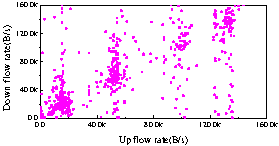
\includegraphics[width=\linewidth]{up-down-rate}
%	\caption{The corresponding rate of upload and download flows.}
%	\label{fig:up-down-rate}
%	\termspace
%\end{figure}

Figure~\ref{fig:up-down-fct} shows the  upload and download flow's corresponding FCT. From the figure we can find that the spots are spread under the lower half part of the figure as the download flows' FCT is shorter than upload flow. And we also find that the sports are discretely spread which means that the download flows' FCT is independent with upload flows' FCT. Figure~\ref{fig:up-rate-down-fct} shows the relationship between the download flows' FCT and the upload flows' rate. Most of the download flows' FCT is short under 200s. The upload flows' rate has not obviously influence to the download flows' FCT as even when the upload flows' rate grows to 100KB/s most of the download flows' FCT is spread under 50s. Figure~\ref{fig:up-down-fct} and Figure~\ref{fig:up-rate-down-fct} confirm that the upload flows' FCT and rate have not obviously influence to the download flows' FCT. So we think the content of the upload video is the key factor that influence the download flows' FCT, which means that viewers determine when to stop watching the video mainly according the video's content. 
%\begin{figure}[ht]
%	\centering
%	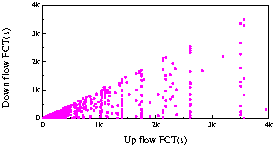
\includegraphics[width=\linewidth]{up-down-fct}
%	\caption{The corresponding flow complete time of upload and download flows.}
%	\label{fig:up-down-fct}
%	\termspace
%\end{figure}

%\begin{figure}[ht]
%	\centering
%	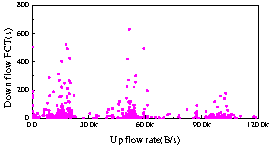
\includegraphics[width=\linewidth]{up-rate-down-fct}
%	\caption{The corresponding download flow FCT with upload flow rate.}
%	\label{fig:up-rate-down-fct}
%	\termspace
%\end{figure}

We also measure what happen in download flow when the upload has stall. We find that 37.2\% stall in upload flows will cause stall in download flow and almost all of these stalls in download flows are  \emph{resource constraint}, the most common stall in download flow. 
%Although we can not match the storage stall with download flows, we think most of the stall in storage flow will also cause \emph{resource constraint} stall in download flows. It is easy to understand as all the stall in upload and storage flows influence the data supply for download flows.














